\documentclass[]{article}
\usepackage{lmodern}
\usepackage{amssymb,amsmath}
\usepackage{ifxetex,ifluatex}
\usepackage{fixltx2e} % provides \textsubscript
\ifnum 0\ifxetex 1\fi\ifluatex 1\fi=0 % if pdftex
  \usepackage[T1]{fontenc}
  \usepackage[utf8]{inputenc}
\else % if luatex or xelatex
  \ifxetex
    \usepackage{mathspec}
  \else
    \usepackage{fontspec}
  \fi
  \defaultfontfeatures{Ligatures=TeX,Scale=MatchLowercase}
\fi
% use upquote if available, for straight quotes in verbatim environments
\IfFileExists{upquote.sty}{\usepackage{upquote}}{}
% use microtype if available
\IfFileExists{microtype.sty}{%
\usepackage{microtype}
\UseMicrotypeSet[protrusion]{basicmath} % disable protrusion for tt fonts
}{}
\usepackage[margin=1in]{geometry}
\usepackage{hyperref}
\hypersetup{unicode=true,
            pdftitle={A deeper look at the relationship between root carbon pools and the vertical distribution of the soil carbon pool: response to reviewers},
            pdfborder={0 0 0},
            breaklinks=true}
\urlstyle{same}  % don't use monospace font for urls
\usepackage{graphicx,grffile}
\makeatletter
\def\maxwidth{\ifdim\Gin@nat@width>\linewidth\linewidth\else\Gin@nat@width\fi}
\def\maxheight{\ifdim\Gin@nat@height>\textheight\textheight\else\Gin@nat@height\fi}
\makeatother
% Scale images if necessary, so that they will not overflow the page
% margins by default, and it is still possible to overwrite the defaults
% using explicit options in \includegraphics[width, height, ...]{}
\setkeys{Gin}{width=\maxwidth,height=\maxheight,keepaspectratio}
\IfFileExists{parskip.sty}{%
\usepackage{parskip}
}{% else
\setlength{\parindent}{0pt}
\setlength{\parskip}{6pt plus 2pt minus 1pt}
}
\setlength{\emergencystretch}{3em}  % prevent overfull lines
\providecommand{\tightlist}{%
  \setlength{\itemsep}{0pt}\setlength{\parskip}{0pt}}
\setcounter{secnumdepth}{0}
% Redefines (sub)paragraphs to behave more like sections
\ifx\paragraph\undefined\else
\let\oldparagraph\paragraph
\renewcommand{\paragraph}[1]{\oldparagraph{#1}\mbox{}}
\fi
\ifx\subparagraph\undefined\else
\let\oldsubparagraph\subparagraph
\renewcommand{\subparagraph}[1]{\oldsubparagraph{#1}\mbox{}}
\fi

%%% Use protect on footnotes to avoid problems with footnotes in titles
\let\rmarkdownfootnote\footnote%
\def\footnote{\protect\rmarkdownfootnote}

%%% Change title format to be more compact
\usepackage{titling}

% Create subtitle command for use in maketitle
\newcommand{\subtitle}[1]{
  \posttitle{
    \begin{center}\large#1\end{center}
    }
}

\setlength{\droptitle}{-2em}
  \title{A deeper look at the relationship between root carbon pools and the
vertical distribution of the soil carbon pool: response to reviewers}
  \pretitle{\vspace{\droptitle}\centering\huge}
  \posttitle{\par}
  \author{}
  \preauthor{}\postauthor{}
  \date{}
  \predate{}\postdate{}

\usepackage{color}
\usepackage{lineno}
\linenumbers

\begin{document}
\maketitle

Anonymous Referee \#1\\
Received and published: 11 April 2017\\
In this study, Dietzel et al. used an agronomic trial to study the
linkage between root C input and the vertical distribution of Soil
Organic Matter (SOM). Using a soil under corn cultivation for more than
a century, they measured the SOM profile of this soil as well as the
root material input and quality (C:N ratio) along the soil depth for
both prairie and maize vegetation. They found that maize allocates a
higher proportion of root input in deep soil layers and that it as a
lower C:N ratio compared to prairie plants, which is quite classical.
Further, they found that root C:N ratio increases with depth for all the
treatments. This result is interesting and quite new from what I know.
This suggests that deeper roots are dominated by transport root with
highly sclerified tissues and poor absorptive proteins content compared
to surface roots. Finally, they conclude that in moving from prairie to
maize, a large, structural-tissue dominated root C pool with slow
turnover, concentrated at shallow depths was replaced by a small,
non-structural tissue dominated root C pool with fast turnover evenly
distributed in the soil profile, suggesting that maize may allocate more
root C input to the soil than prairies at deeper depths. This
constitutes the strong portion of this manuscript.

\textcolor{blue}{Thank you, we too were excited to quantify differences in prairie and maize root allocation and find root C:N ratios increase with depth.}

Based on the conceptual framework and the empirical results of the study
of Cotrufo et al. (2015) about the formation of SOM, they also argue
that their pattern of increasing root C:N ratio with depth could explain
why an disproportionally large stock of SOM relative to root C inputs is
found in deep soil. First, I found it quite tricky to conclude about the
driver of such a global scale pattern from data of a case study like
this.

\textcolor{blue}{Yes, since this is only one study, we avoid making any strong conclusions, but do suggest that root C:N ratio plays a role in development of the soil profile. Finding increases in root C:N ratios with depth is significant on its own, but we feel it is very important to put this finding in the context of larger scientific questions.}

Beyond that, I am not convinced by this interpretation and I found their
argumentation about this statement quite weak for several reasons
related to logical contradiction and some misunderstanding about the
work of Cotrufo as discussed into more detail below.

\textcolor{blue}{We feel we can do a better job communicating our proposed mechanism and we address these details below. We found your comments to be extremely helpful towards improving this manuscript and enjoyed getting a new perspective on many of the aspects we have wrestled with during writing. It seems we all have the same understanding of Cortrufo et al.'s conceptual models, but are used to thinking about these models under different environmental circumstances. One major assumption on which we do not completely agree is the likeliness of microbial by-products to be transported deeper in the soil profile. We hope the discussion below and additional references help to clarify the manuscript.}

If I consider these two paths of SOM formation and your results
together, I would consider that shallow root of high litter quality
would supply high input of DOC that can be efficiently processed by soil
microorganisms (high Carbon Use Efficiency {[}CUE{]}) and supply larger
quantity of microbial by-products that can be then stabilized in soil
microagregates by mineral-binding, thus leading to higher C
sequestration. In contrast, the deep root of poor quality (higher
proportion of POM) will be least efficiently processed, thus leading to
higher C lost by mineralization relative to SOM formation and ultimately
lower C sequestration. This is thus not consistent with the pattern of
the disproportionally large stock of SOM relative to root C inputs in
deep soil.

\textcolor{blue}{Right! We find this inconsistency in patterns very interesting and a major motivation for the manuscript. Although the proposed relationship we describe between root C:N ratio and soil C profile development is not immediately intuitive, the combination of MEMS and dissolved organic carbon (C) transport leads to a very possible mechanism behind a disproportionally large stock of SOM relative to root C inputs.}

Further,Cotrufo et al. (2015) studied SOM formation over short-term
scale whereas deep soil C is often hundreds to thousands year-old and
highly microbialy processed.

\textcolor{blue}{Yes, Cortrufo et al. have focused on short-term scales and their conceptual model is still hypothetical, however, what happens in the short-term is directly connected to what happens in the long term. The fact that deep soil C is highly microbially processed does not indicate where where the C originated.}

Fontaine et al. (2007) found that deep soil C mineralization is strongly
limited by energetic constraints. This slow turnover together with the
DOC input from surface to deep soil layer documented by Rumpel and
Kögel-Knabner (2010) could more likely explain the disproportionally
large stock of SOM relative root C input is found in deep soil.

\textcolor{blue}{Both of these factors, and many more mentioned in the manuscript, contribute to the disproportionally large stock of SOM relative to root C input found in deep soil, but do not fully explain it and do not incorporate the role of root C:N ratio. The transport of DOC is especially important in our proposed mechanism and we spend some time on how roots at shallow depths vs. deeper depths contribute to this DOC.}

I also pointed several methodological issues detailed below. Finally, I
fell that you did not so much discussed how the root system of your
different plant communities (maize vs.~prairie) could explain the
vertical C profile of your studied soil though this constitutes the
strong part of your study to the linkage between root C input and the
vertical distribution of SOM.

\textcolor{blue}{Thank you for the methodological questions below. We would have liked to spend more discussion on the root systems of maize vs. prairie, but felt that without measurements of the original soil C profile, discussion specific to change created by annual cropping systems would be challenged. However, we can strengthen this component in response to your comment.}

Taken together, I think this manuscript will need important revisions to
be acceptable for publication, especially by avoiding tricky
extrapolation and misinterpretation and by refocused on the conclusion
you can reasonably draw from your results. Clarify your scientific
questions/hypotheses could also help to achieve this end.

Detailed discussion of the manuscript

P.1-L. 15. `in moving from prairie to maize' If ?? I well understood
your design, you studied soil root allocation on restored prairies that
have maize cropping historical of \textgreater{}100 years. Therefore,
would it not be more correct to talk about moving from maize to prairie.

\textcolor{blue}{We are referencing the historical shift from prairie to maize. I will change the wording for clarification.}

P.1-L. 15. `contribute' to what? To soil C stock? Please clarify.
Alternatively, we could also talk about `C allocation'.

\textcolor{blue}{Yes, soil C stock. We will clarify}

P.1-L. 21. Please clarify what you mean by `aboveground process'. Is
really soil disturbance (tillage?) an aboveground process?

\textcolor{blue}{Will change 'aboveground processes' to 'soil management'.}

P.1-L. 26-27. Is this definition really necessary here? I think it will
be better placed in the Material and Methods section.

\textcolor{blue}{We included it here as we go on to use the definition in the introduction.}

P.2-L.5. Please insert the Weaver citation

\textcolor{blue}{Thanks for catching this, we will insert the citation.}

P.2-L.17. Why did you used `Carbon:N' though you used `C:N' just before.

\textcolor{blue}{We did not want to start a sentence with an abbreviation.}

P.2-L.19-21. I do not clearly see how your experimental design give you
a `unique perspective on characteristics of root inputs' Please clarify.

\textcolor{blue}{We expect many of the characteristics reported here to be less detectable in well-established prairies systems, but you are right that prairie reconstruction in not entirely unique. We will replace "unique perspective" to "new perspective".}

It would also be useful to indicate here the number of year since
prairie restoration at the end of the study (5 years not?).

\textcolor{blue}{Yes, this will be added here.}

P.2-L.26-27. I did not understand the point of your second scientific
question before to read the last extion of your discussion. Please be
not explicit and precise on your purpose.

\textcolor{blue}{Thanks for this comment. You illustrate that we need to change some aspects of the introduction to make it understandable for an international audience. For example, in this instance we will simply say "perennial prairie" instead of "historical" and "annual cropping systems" instead of "current systems".}

P.3-L.1-2. What about soil N concentration? This could be importabnt

\textcolor{blue}{We do have total soi N data and will include it here.}

P.3-L.1-2. How many replicates (blocks)? 4? This information is crucial!

\textcolor{blue}{I'm sorry we did not include this, it will be added.}

P.5-L.4-8. You used linear mixed models. Please state what factors are
formulated as fixed or random effects in your models.

\textcolor{blue}{This information will be added.}

P.5-L.15-23. Logistic model is used fit binary response variable.
Therefore, I do not see the rationale to use Logistic model to fit root
mass, which is a continuous variable. . .

\textcolor{blue}{We will add more details here. Logistic regression is used to fit binary response variables. We used a logistic function to fit the data and then statistically compared the parameters of each fit of the function as described in the book "Mixed Effect Models in S and S-plus", Pinheiro and Bates, 2000. We will add this citation.}

P.5-L.19. It is not so clear to me what you mean by ``root mass
accumulation''. It is the difference in root mass between two sampling
dates? Or is it cumulative root growth? But you did not measure it
between all sampling dates, right? Please clarify. By the way, it not so
clear what was the initial root mass stock and distribution prior to
experimental set-up.

\textcolor{blue}{"Root mass accumulation" refers to root mass gained. We did not measure it between all sampling dates, rather we used the model we fit to predict values during times we did not make measurements.}

P.5-L.29-30. We calculated root turnover constant as k = root loss /
root stock. This computation is quite uncommon. Hence, Gill and Jackson
(2000) calculated root turnover constant as k = root gain / root stock.
In addition to be more standard method, I also found it clearer as root
gains are directly obtained with the ingrowth core method while your
root loss computation use root mass accumulation, which was not very
well defined.

\textcolor{blue}{We can and will easily replace "root loss" with "root gain" in our equation.}

P.7-L.9. Throughout the manuscript, we heavily use the `pool'. Though I
found this term appropriate for distingue different component of the
global soil C stock, I found the term `stock' more suitable when talking
about quantitative estimate.

\textcolor{blue}{We will change the text so that 'pool' is used only when discussing specific components of the global soil C stock.}

P.6-L.6. There is no reference to Table 1 in the text.

\textcolor{blue}{Our apologies, we will correct this.}

P.11-12. There is no reference to most of your tables and figures in
this portion of your result section. . . You really need to clearly use
reference to it for justify what you state in the text. In its current
state, I do feel really difficult to follow your text.

\textcolor{blue}{We will add more references to make the text easier to follow.}

P.10-Table 3. Is this really useful ? Figure 4 already provide this
information. This table should be place in appendix. By the way, I found
that there is quite too much table and figure in the article.

\textcolor{blue}{We will be happy to move Table 3 to the appendix and consider removing or combining some of the figures.}

P.11-L.15. What you mean by input? Is it your root mass accumulation?
Please clarify.

\textcolor{blue}{Root mass accumulation is root mass input - root mass loss. Input is how much root mass went into the soil. We will clarify this in the text.}

P.12-L.6. What about soil N concentration and soil C:N ratio across soil
depth and treatment? Isn't this information important is understand the
root C:N profiles?

\textcolor{blue}{Yes, this information is important and we can include total (organic + inorganic) N values for this soil. While root C:N ratio increases with depth, soil C:N ratio decreases with depth, and it may be useful to discuss this relationship.}

P.13-L7-8. `a physical-transfer pathway whereby plant tissue is
processed by soil microbes to its fullest extent, and then remains in
the soil functionally inert'. Really? Cotrufo et al. (2015) actually
talk about physical transfer of Particulate Organic Matter (POM) from
litter to soil. POM is not functionally inert!

\textcolor{blue}{We will change this to better reflect Cotrufo's original language and refer instead to the "inherent chemical recalcitrance" of organic matter resulting from the physical-transfer pathway.}

P.13-L.11-19. `root decomposition in our study would have resulted in a
gradient of microbially-derived to physically-derived organic matter
from the top of the soil profile downward' Then this is not consistent
with evidence that the contribution of microbial- and not root-derived C
increases with depth (Rumpel and Kogel-Knabner, 2011) in contrast with
what you stated L.15-16.

\textcolor{blue}{The sentence following this one in the manuscript is very important. The microbially-derived organic matter would be mobile and transported to deeper depths, contributing to the relatively immobile pool of physically-derived organic matter. This is very consistent with Rumpel and Kogel-Knaber (2011), as we eventually conclude.}

I assume that DOC derived from soil surface can be mobile and move down
the profile but a large portion can be stabilized in the surface and at
least the SOM derived from deep root with high C:N ratio should be less
microbial-derived given what you state. This point should be clarify.
Moreover, the notion physically-derived SOM does not make sense, see my
previous comment.

\textcolor{blue}{Yes, DOC can be stabilized in the soil surface, but the proportion of C stabilized depends on soil type and level of C saturation. We will add a reference to Castellano (2015) to support this idea. These prairie-formed soils do not have C concentrations as high as historical levels, but total C concentrations are still at 2.8 percent, indicating a reduced capacity for additional C stabilization. In this environment, microbial by-products are likely to be part of the soil solution and easily transported to deeper depths with greater capacity for C stabilization. We will make this clearer in the manuscript.}

P.13-L.12-14. `Soil organic matter at the soil surface would be
vulnerable to transport to greater depth as dissolved organic C whereas
physically-transferred soil organic matter at depth would be relatively
immobile'. If you read carefully Cotrufo (2015), she stated that DOC
derived from litter is preceded by soil microorganisms and the microbial
by-products are then stabilized in soil microagregates by
mineral-binding. This mineral-stabilized SOM is thus actually less
mobile than POM, in contrast with what you stated.

\textcolor{blue}{Microbial by-products are very mobile until they are stabilized. When and where they are stabilized depends on the soil conditions. In the mechanism we propose, microbial by-products reach the deeper profile and are stabilized there. This is consistent with findings that proportion of microbial-derived SOM increases with depth.}

P.13-L.16-19. Exsudates are highly labile compounds that are very
quickly preceded by soil microorganisms. Once metabolized, they are much
less mobile. Therefore, they probably represent a minor fraction DOC
moving down the profile and that could form deep SOC.

\textcolor{blue}{Thank you, we should provide clarification that exudates quickly move into microbial pools. However, the fate of the C after that again depends on the environmental capacity for microbial by-products to be stabilized.}

P.13-L.27-29 `By the sixth year of reconstructed prairie establishment,
root C pool equilibrium was reached and prairies began making
substantial annual contributions to the soil organic matter pool above
30 cm, although the fraction of organic matter that remained in the soil
is unknown' You have information on root litter decomposition and soil
organic matter turnover, so cannot state anything about SOM formation or
stock. All you can saw this you likely have higher root litter input
that could eventually increase SOM stock.

\textcolor{blue}{You are absolutely right. This will be fixed by changing 'contributions' to 'inputs'.}

P.13-L.35-37. Probably, but this is quite speculative. . .

\textcolor{blue}{It is indeed speculative, but the most reasonable answer given the evidence available.}

P.14-L.10. `contributed more C' This is unclear.

\textcolor{blue}{Will change to 'had greater C inputs'.}

References Cotrufo, M. F., Soong, J. L., Horton, A. J., Campbell, E. E.,
Haddix, M. L., Wall, D. H. \& Parton, W. J. (2015) Formation of soil
organic matter via biochemical and physical pathways of litter mass
loss. Nature Geosci, 8, 776-779.

Fontaine, S., Barot, S., Barre, P., Bdioui, N., Mary, B. \& Rumpel, C.
(2007) Stability of organic carbon in deep soil layers controlled by
fresh carbon supply. Nature, 450, 277-U10.

Gill, R. A. \& Jackson, R. B. (2000) Global patterns of root turnover
for terrestrial ecosystems. New Phytologist, 147, 13-31.

Rumpel, C. \& Kögel-Knabner, I. (2010) Deep soil organic matter a key
but poorly understood component of terrestrial C cycle. Plant and Soil,
338, 143-158.

\textcolor{blue}{Castellano, M. J., Mueller, K. E., Olk, D. C., Sawyer, J. E. and Six, J.: Integrating plant litter quality, soil organic matter stabilization, and the carbon saturation concept, Global Change Biology, 21(9), 3200-3209, doi:10.1111/gcb.12982, 2015.}

\begin{center}\rule{0.5\linewidth}{\linethickness}\end{center}

Anonymous Referee \#2\\
Received and published: 17 April 2017

Dietzel et al. report on a root study conducted at a field experiment
where continuous corn is compared to reconstructed fertilized and
unfertilized prairie stands. They have measured: 1) root profiles to
depth of 1 m at the end of the growth season for six consecutive years,
2) root production (by regrowth cores) for 2 growing seasons to 30 cm
depth, 3) root and soil C and N concentrations to 1 m depth. Extracting
root for multiple growing seasons, multiple soils layers and multiple
replicated treatments is by no mean easy, and the soil science community
can certainly benefit from such precious data. The authors report
interesting findings: 1) the C/N ratio of root material increases with
depth, which has potential implications for soil C storage, 2) the maize
root profile is more uniform with depth than that of prairie species
(confirmative), 3) fertilization of the reconstructed prairie greatly
decreases root biomass.

However, I have some significant concerns with the study:

\begin{enumerate}
\def\labelenumi{\arabic{enumi})}
\tightlist
\item
  The continuous accumulation of maize roots throughout the 6-year
  period is quite troubling (Fig A3). The authors provide one reference
  (Dupont 2014) stating that intact prairie root (not maize) can be
  found in soil several years after cultivation. However, they ignore
  the substantial literature on maize roots that clearly indicates that
  maize roots decompose rapidly in soils, starting with the classical
  study of Mengel and Barber in 1974 (Agron. J. 66: 341-344) and several
  studies that have followed. Actually, Mengel and Barber (1974) state
  that root length and fresh weight decrease rapidly after maize has
  reached the reproductive stage. Here, Dietzel et al. themselves state
  in the abstract about maize roots that they are
  ``non-structural-tissue dominated root C pool with fast turnover''.
  They also indicate that the site was apparently under maize soybean
  rotation prior to starting the experiment, so why was there no
  accumulated maize root biomass at the start of the experiment (if the
  root accumulation theory is correct)? Unfortunately, in the present
  study the roots were not sampled at the same time each year (from
  early October to early November), and the accumulation of maize roots
  the last two years also corresponds to the 2 earliest sampling. A
  possible explanation is that the roots actually decomposed quickly in
  the field and that by sampling a month earlier by the end of the
  six-year period a greater number of non-decomposed roots were
  retrieved. Effects of inter-annual climatic variability on root growth
  is another potentially contributing effect. There are three
  implications from this: 1) apparent maize-root accumulation in the
  field over 6 years is probably an artefact, 2) the pool and rate
  modelling of Fig 3 and 4 is not justified (it did not bring much to
  the paper anyway), 3) the paper should have included a much more
  throughout review of the literature about maize-root dynamics in field
  soils.
\end{enumerate}

\textcolor{blue}{Thank you very much for bringing this to our attention. The possibility of such as artifact led us to additional analysis of our data. During this analysis, we found that the dates included in the methods section were not correct. We are very sorry for this mistake. Please find below a figure that illustrates that time of sampling was most likely not a contributing factor in the accumulation of root mass.}

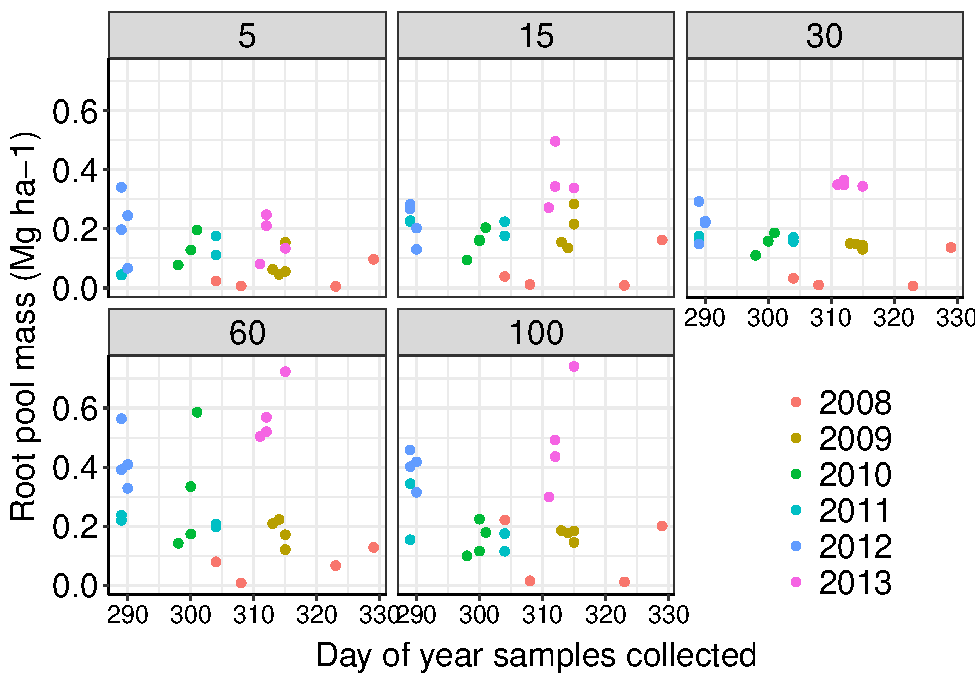
\includegraphics{Response_to_reviewers_files/figure-latex/sampling time-1.pdf}

\textcolor{blue}{You bring up some other useful points here, thank you. We can certainly include more papers on the decomposition of maize roots. Our values for maize biomass taken after maize harvest are typically ~10 percent of maize root values taken at maturity. This is in line with studies that have found that maize roots decompose rapidly. However, decomposition rate is an exponential function, with rapid decomposition occurring early and a slower rate of decomposition occurring later. Several months after maize maturity we are most likely sampling during a period of slower root decomposition.}

\textcolor{blue}{We also questioned the lack of accumulated root mass from years previous to our experiment. We were careful to collect maize root samples 20 cm from our maize row and to plant our rows within 2-3 cm of the previous year's row. We assumed that the cropping legacy from years past would have left a more homogenous distribution of roots than the one we implemented.}

\begin{enumerate}
\def\labelenumi{\arabic{enumi})}
\setcounter{enumi}{1}
\tightlist
\item
  The maize-root C profile is presented 3 times in the paper: 1) Fig 1
  b, 2) Fig 2, and
\item
  Fig. A3. The 3 figures are in the same units (Mg ha-1), but I could
  not reconcile the data between them. The 2013 data of fig. 1 b (with
  largest root accumulation in the top soil) do not seem to correspond
  to the 2013 data of figure A3, which seems to show highest maize-root
  biomass in the deeper soil.
\end{enumerate}

\textcolor{blue}{You are correct in not being able to reconcile the figures in the paper (1b and 2) with the figures in the appendix (A3) because the depth increments are not the same. Figure A3 shows the actual data, mass collected at 0-5, 5-15, 15-30, 30-60, and 60-100 cm depths. For example, the deepest depth increment is 40 cm long, resulting in high values relative to 5-15 cm, only 10 cm long. We used the values taken in these depth increments to break distribution into 5 cm increments, as described in P6, L 3-4. This gave a more accurate depiction of the distribution of both roots and organic C through the soil profile, shown in Figs. 1 and 2.}

In addition, the maize root profile appears more even in Fig.2 than in
Fig. 1 b, while it should be exactly the opposite (e.g.~the 5-10 cm
should have about half of the 0-5 cm in fig 2, if extrapolated from fig
1). Or are the two figures exactly the same? But why figure 2 then? The
3 figures should have been reconciled and presented as one main figure
in logical units, and then the results compared to the literature.

\textcolor{blue}{Fig. 1b and Fig.2 are drawn from the same dataframe. Fig. 1 shows distribution patterns that, as you point out, are not visible in Fig. 2, especially for maize. We use Fig. 1 to discuss root and soil C distribution in the soil profile. Figure 2 shows absolute differences in root pool mass among treatments, not visible in Fig. 1. Fig. 2 is used to point out and discuss these basic differences.}

\begin{enumerate}
\def\labelenumi{\arabic{enumi})}
\setcounter{enumi}{2}
\tightlist
\item
  Data from the root regrowth cores are not clearly presented, but used
  for a direct extrapolation of a root turnover rate in the top 30 cm.
  Summary data (without statistics) are presented in g m-2 in Table 4,
  making it difficult to compare to the root pool data presented in Mg
  ha-1. The maize root productivity appears low and I am missing a
  coherent evaluation of the C input in the context of published
  studies.
\end{enumerate}

\textcolor{blue}{Sorry these data are not clear, we will improve this in the paper as well as change the units to correspond with other reported units. The maize root productivity is low because samples were taken 2-3 months after maize maturity, which we will also highlight.}

\begin{enumerate}
\def\labelenumi{\arabic{enumi})}
\setcounter{enumi}{3}
\tightlist
\item
  The implications for C storage presented in this paper are largely
  hypothetical and somewhat contradictory. The present paper contains no
  significant result to link root biomass profiles to soil C profiles.
  While it is OK to briefly elaborate about possible implication of a
  higher root C/N ratio with depth, this should not be the main part of
  the discussion, which should instead focus on actual significant
  results.
\end{enumerate}

\textcolor{blue}{The implications for C storage presented in this paper are partly hypothetical, but are complex and novel enough to warrant extensive discussion. The mystery of the disproportionally large stock of SOM relative to root C input found in deep soil has been unsolved since first noticed over 100 years ago and root C:N ratio increase with depth is a new and useful piece of information. We do not have direct evidence to link root biomass profiles to soil C profiles, but what we do have, combined with what we are able to model, is better than anything that has been previously published.}

In addition, I could not reconcile the two ideas presented here about
the effect of root C/N ratio on C storage in soils. On the hand, the
authors argue that a lower C/N ratio for maize root favours C storage in
soil as compared to prairie roots (p14, line 11-12). On the other hand,
they also argue that an increasing C/N ratio of roots with depth in the
soil profile also favours C storage (e.g.~p1, line 10-12). The potential
attempt to reconcile these two contradictory effects of root C/N ratio
on soil C was unconvincing (p 14).

\textcolor{blue}{We will reword P1, line 10-12 - "In all treatments we found that root C:N ratios increased with depth, which may help explain why an unexpectedly large proportion of soil organic C is found below 20 cm." It is meant to suggest that increaseing C:N ratios with depth play a role in an unexpectedly large proportion of soil organic C found below 20 cm, not that the increase in C:N ratio directly contributes C storage. The relationship between C:N ratios and C storage is not necessarily intuitive, as we later describe in the text.}

In conclusion, Dietzel et al. have collected an impressive data set on
maize and prairie roots following maize-soybean rotation. The dataset
appears to suffer from some artefacts, but root studies are difficult
and shortcomings could have been acknowledged.

\textcolor{blue}{Thank you.}

The data themselves are neither clearly presented nor sufficiently
discussed in light of the literature. A main finding is largely ignored,
i.e.~the dramatic reduction of root biomass by fertilization in prairie
systems.

\textcolor{blue}{Indeed, apart from the figures, we did include only three sentences on this finding. The effect of N fertilization on perennial root biomass is well-known (Troughton 1960, Thornley 1972, Gregory 2007) and we did not consider this plant response to be particularly important to a soils audience.}

By contrast, the authors focus on an uncertain modelling and
non-verifiable considerations about the effect of root C/N ratio on soil
C. A focus on significant results and discussion of these results in
light of the literature would have better served this study

\textcolor{blue}{While modelling is always uncertain, the fits of the models we used were very good and we stand behind the conclusions drawn from this effort. The effect of root C:N ratio on soil C may never be verifiable because it is a centuries-long process that is difficult to measure, but root C:N ratio plays some role in the development of the soil C profile. This manuscript is the very first to question this role and work with existing data to propose a mechanism by which root C:N ratio contributes to soil C profile development. It is our hope that by focusing our paper on root C:N ratios and current soil C profiles, we are inspiring and supporting future studies that will examine this important relationship more closely. Merely commenting on this possible relationship in a manuscript focused on a comparison of maize and prairie roots would not reach the intended audience or provide direction for related experiments.}

\textcolor{blue}{Gregory, P.: Plants Roots: Growth, Activity and Interaction with Soils, in Plant, Roots and the Soil, pp. 5-7, Blackwell Publishing Ltd., 2007.}\\
\textcolor{blue}{Thornley, J. H. M.: A balanced quantitative model for root: shoot ratios in vegetative plants, Annals of Botany, 36(145), 431-441, 1972.}
\textcolor{blue}{Troughton, A.: Further studies on the relationship between shoot and root systems of grasses, Journal of
the British Grassland Society 15, 41-47, 1960.}
\_\_\_\_\_\_\_\_\_\_\_\_\_\_\_\_\_\_\_\_\_\_\_\_\_\_\_\_\_\_\_\_\_\_\_\_\_\_\_\_\_\_\_\_\_\_\_\_\_\_\_\_\_\_\_\_\_\_\_\_\_\_\_\_\_\_\_\_\_\_\_\_\_\_\_\_\_\_\_\_\_\_\_\_\_\_\_\_\_\_\_\_
M. W. I. Schmidt
\href{mailto:michael.schmidt@geo.uzh.ch}{\nolinkurl{michael.schmidt@geo.uzh.ch}}
Received and published: 11 April 2017

\emph{A note upfront from the submitting person: This review was
prepared by Nadja Huber and Mirjam Mächler, both master students in
geography at the University of Zurich. The review was part of an
exercise during a second semester master level seminar on ``the
biogeochemistry of plant-soil systems in a changing world'', which I
organize. We would like to highlight that the depth of scientific
knowledge and technical understanding of these reviewers represents that
of master students. We enjoyed discussing the manuscript in the seminar,
and hope that our comments will be helpful for the authors.}

\textcolor{blue}{That is so great that you discussed our paper as a group! What a great exercise and these comments are just the sort of thing we hoped would happen when submitting a paper to Soil. Thanks a lot for your comments. Hearing from many people really makes obvious which portions of the paper are difficult to understand and where the most improvement is needed.}

Dietzel et al. start with the fundamental statement, that soil organic
carbon and root mass are disproportionately distributed in soils,
supposing that root mass has a direct influence on soil carbon pool. As
a matter of fact, in a depth below 20cm half of all soil organic C in
soils can be found where just a third of all root mass is. There is no
clear answer to the question, why there is such a large difference
between the two C pools. Dietzel et al. mention that temperature,
moisture, O2, soil texture and soil C values are part of the explanation
of this discrepancy. Still, the C:N ratio as part of it has always been
neglected in previous studies.

\textcolor{blue}{Indeed, decreases in root C:N ratio with depth has been an unknown factor.}

The paper therefore specifically concentrates on a more detailed look at
the properties of C pools. For this purpose the authors examined soil C
and root C pools in three different cropping systems. Continuous maize,
multispecies prairie and N-fertilized multispecies prairie. Research
questions asked were the following: ``1) How does the quantity,
distribution, and C:N ratio of the root C pool differ with depth and
between these native perennial and non-native annual ecosystems and 2)
what do these differences in input tell us about the historical
belowground ecosystem under which these soils developed and the systems
and will these soils continue to change?'' To answer these questions the
authors conducted a field experiment over six years in Boone County, IA,
USA. With this field experiment the authors were able to show that an
increase in root C:N ratio with depth is a potentially important factor
determining the distribution of C in the soil profile. The authors
consider the root pool C:N ratios to be sufficiently important that they
result in a greater maize C contributions to soil organic matter than
prairie C below 20 cm.

Objective 1 (root quality and quantity with depth) was discussed in
detail in the manuscript.

During the discussion in the classroom, however, it became clear that
objective 2 and the related discussion confused all of us. We did not
understand i) why the ``historical belowground ecosystem'' is important

\textcolor{blue}{Reviewer 1 also brought this to our attention. This sentence needs to be reworded to be more explicit for a broader audience. The 'historical belowground ecosystem' is the prairie systems under which the soils formed.}

and ii) how objective 2 relates to the presented results. The question
if these soils will continue to change is rhetoric (soil always continue
to develop) and very unspecific.

\textcolor{blue}{Yes, this part of the sentence will also be reworded. We did not mean 'if', but 'how' soils will continue to change under annual cropping systems compared to reconstructed perennial systems.}

The corresponding discussion section (4.3) is very short and
speculative. Are root ``turnover'' (with a lifetime of a few years) and
soil organic carbon turnover (decades to centuries) somehow related?

\textcolor{blue}{They are definitely related. Where does soil organic carbon come from? As roots cease to be roots, they turn into CO2 or organic matter, influencing soil organic carbon turnover on the scale of days to centuries, even thousands of years for soils that have been occupied by roots for thousands of years.}

Probably they are not. Coincidence is not causation. We wondered if
objective 2 and section 4.3 are needed at all. If you think they are,
please elaborate this part of the manuscript.

\textcolor{blue}{Yes, we will certainly elaborate on this.}

Detailed comments: We did not fully understand the link between C:N and
root depth. Do you mean that C:N ratios increase with depth depending on
species or on individual plants?

\textcolor{blue}{As we move deeper into the soil, root C:N ratios increase for all plants in this study.}

P. 3, line 26: what does ``sampling by replicate block from 31
October-25 November 2008'' mean? Did you sample repeatedly? Explanation
of ``replicate block''-approach needed.

\textcolor{blue}{Yes, this is not clear and we will add more details.}

P. 4, line 11/12: is there a difference between root measurements and
root data?

\textcolor{blue}{Yes, there is. We should not have used them interchangeably here. Thanks for catching that.}

P. 4, line 24/25: why different storage? Further explanation desired.

\textcolor{blue}{We explain that storage was different because soil from the first year was part of an incubation experiment.}

P. 5, line 28: why the period between April 1st and November 30th to
calculate the average root mass accumulation? Are these official dates?
Further explanation needed.

\textcolor{blue}{These dates are the approximate window for plant growth in our region. We will include that information in the manuscript.}

Table p.~10: unclear -\textgreater{} explanation of upper/lower case
letters and meaning of those letters is missing; it could be part of the
description of the table

\textcolor{blue}{This information is in the caption. Perhaps it did not come through with the format you were looking at.}

Explanation pro glimmix on page 5/14 but not in table description.

\textcolor{blue}{Thank you, but not sure what you are looking for here.}

P. 13, line 3: increase in root pool C:N ratio has not been reported
previously in the literature: We would appreciate some information about
previous research which focused on a related topic

\textcolor{blue}{We literally could not find any literature related to root pool C:N ratio.}

P. 14, line 3/4: the pattern of distribution of what? Do you mean the
vertical distribution of roots? What is place in this context?

\textcolor{blue}{Pattern of distribution of roots. We will add this to the text.}

P. 14, line 30-32: For us, this sentence is very long and difficult to
understand. No significant changes in soil C (changes in quantity or
stocks?) at any depth but differences in quantity?

\textcolor{blue}{We will split this sentence up into segments that are easier to understand. No changes in soil C despite changes in root quantity.}

``implementation of annual cropping systems'': Do you refer to line 19?
Experimental location was a site of cultivation under annual crops for
over 100 years.

\textcolor{blue}{These soils were dominated by prairies for ~10,000 years, so the shift to annual cropping systems 100 years ago is still relatively recent in terms of soil development. This information is important for us to add to the text.}

Remarks concerning formal structures (typos, figures etc.):

P. 3, line 2: typo: 11 mg kg-1

\textcolor{blue}{Thanks.}

Figure p.~6: why not making a title with total C, root C maize, etc.
instead of letters a,b,c -\textgreater{} would be more clear and
consistent with the following figures

\textcolor{blue}{Yes, we can change this.}

Figures p.8 + 9: legend can be improved -\textgreater{} no units
-\textgreater{} unclear \& colors are not suitable for black/white
printing

\textcolor{blue}{We will add units to the legend and we used to different linetypes for different treatments in black and white printing, but see now that is not obvious.}

P. 13, line 36: typo: this

\textcolor{blue}{Thanks.}


\end{document}
